In December 2012 software engineer Cheng Zhao joined GitHub's team, having previously worked for Intel developing
node-webkit, with the task of porting the Atom editor from using Chromium Embedded Framework to node-webkit.
Node-webkit being a Node.js module developed by Roger Wang which combined the browser engine used by Chromium - WebKit - 
with Node.js, making Node.js modules accessible from JavaScript code running inside a web page. \parencite{jensen2017}\paragraph{}

Porting to node-webkit proved difficult, so GitHub abandoned that approach, and it was decided that a new native shell
for Atom would be created.
Said shell was dubbed \emph{Atom Shell} and after development was finished and the Atom editor was open sourced
by GitHub, Atom Shell soon followed suit and was renamed to \emph{Electron}.
Initially developed as a way to deliver an editor, numerous widely known applications like Slack, Discord and Visual
Studio have started using Electron to develop and deliver their desktop applications.\parencite{electronDocs}
But what exactly is Electron?\paragraph{}
Electron is a framework which allows for the development of cross-platform desktop applications using only popular 
web programming languages like HTML, CSS and JavaScript. 
While the advantages will be discussed in detail in the next chapter \emph{Why Use Electron?}, the appeal to developers
is obvious: Maintaining one codebase while being able to deliver the app to all desktop operating systems.\paragraph{}
Now, as described previously the Electron framework serves the same purpose as node-webkit (later renamed to NW.js), but
their approaches do differ in certain ways: \parencite{jensen2017}\par
\begin{figure}[ht]
    \label{fig:el-architecture}
    \caption{A simplified representation of Electron's architecture. \parencite{jensen2017}}
    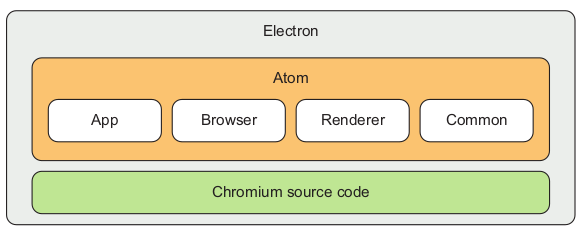
\includegraphics[width=\textwidth]{electron-architecture}
\end{figure}
Without going into detail on how NW.js works, Electron and NW.js share some architectural similarities.
However, there are some differences in how Electron combines Node.js with Chromium.\paragraph{}
Architecturally, Electron places an emphasis on strict separation from Chromium source code, ass seen in figure \ref{fig:el-architecture}.
This looser integration allows for easier updates to the Chromium part of the source code, whereas with NW.js Chromium
is patched to allow for Node.js and Chromium to use a shared Javascript state. \parencite{jensen2017}\par
On the other hand, this means that Electron has separate JavaScript contexts: A \emph{main} process which starts running
with the app window and a \emph{renderer} process for each individual window.
Any sharing of state between these contexts, or simply put between the front- and back-end, has to pass through the
\emph{icpMain} and \emph{icpRenderer} modules.
This means that each JavaScript context is kept separate but data can be explicitly shared, allowing for greater control
over what state exists in which app window. \parencite{jensen2017}\paragraph{}
Electron itself (the part without Chromium) is made up of for different components: App, Browser, Renderer and Common.
\textbf{App} contains code written in C++ and Objective-C++ responsible for loading Node.js and Chromium's content module.
The \textbf{browser} folder contains code which handles interactions with the front-end.
This is to say functionality such as loading the JavaScript engine, interacting with the UI and binding operating system
specific modules.
As for \textbf{renderer}, this component handles the different renderer processes.
Because Chromium works by running each tab as an individual process, as to not crash the entire browser should one
tab become unresponsive, each application window in Electron runs as its own process.
\textbf{Common} contains code which is used by both the main and renderer processes for running the application.
Among other things this folder also contains the integration of Node.js' event loop with Chromium's event loop. \parencite{jensen2017}\paragraph{}
